\documentclass{beamer}
\usepackage{ctex}
\usepackage{listings}
\usepackage{algpseudocode}
\usepackage{graphicx}
\usepackage{geometry}
	\usepackage{fontspec}
	\setmonofont{Consolas}
\usepackage{xcolor}
\lstset{
    columns=fixed,    
    basicstyle=\ttfamily\scriptsize,   
    numberstyle=\tiny,
    numbers=left,                                        % 在左侧显示行号
    frame=none,                                          % 不显示背景边框
    backgroundcolor=\color[RGB]{245,245,244},            % 设定背景颜色
    keywordstyle=\color[RGB]{40,40,255},                 % 设定关键字颜色
    numberstyle=\footnotesize\color{darkgray},           % 设定行号格式
    commentstyle=\it\color[RGB]{0,96,96},                % 设置代码注释的格式
    stringstyle=\rmfamily\slshape\color[RGB]{128,0,0},   % 设置字符串格式
    showstringspaces=false,                              % 不显示字符串中的空格
    language=c++,                                        % 设置语言
}
\expandafter\def\expandafter\insertshorttitle\expandafter{%
	\insertshorttitle\hfill%
	\insertframenumber\,/\,\inserttotalframenumber}
\usetheme{warsaw}
\author{罗昊}
\title{编译实习分享}
\institute{https://github.com/vangohao/hcc}
\begin{document}
 
\frame{\titlepage}
 
\begin{frame}[c]\frametitle{Eeyore 简介}
\begin{enumerate}
\item 使用flex,bison和C++构建,将输入的MiniC代码转换为Eeyore三地址代码.
\item 使用STL的map模板制作符号表,使用链表串联内外层程序块的符号表.
\item 使用回填法构建eeyore中的标号及goto语句.
\end{enumerate}
\end{frame}
\begin{frame}[c]\frametitle{Eeyore 语法结构}
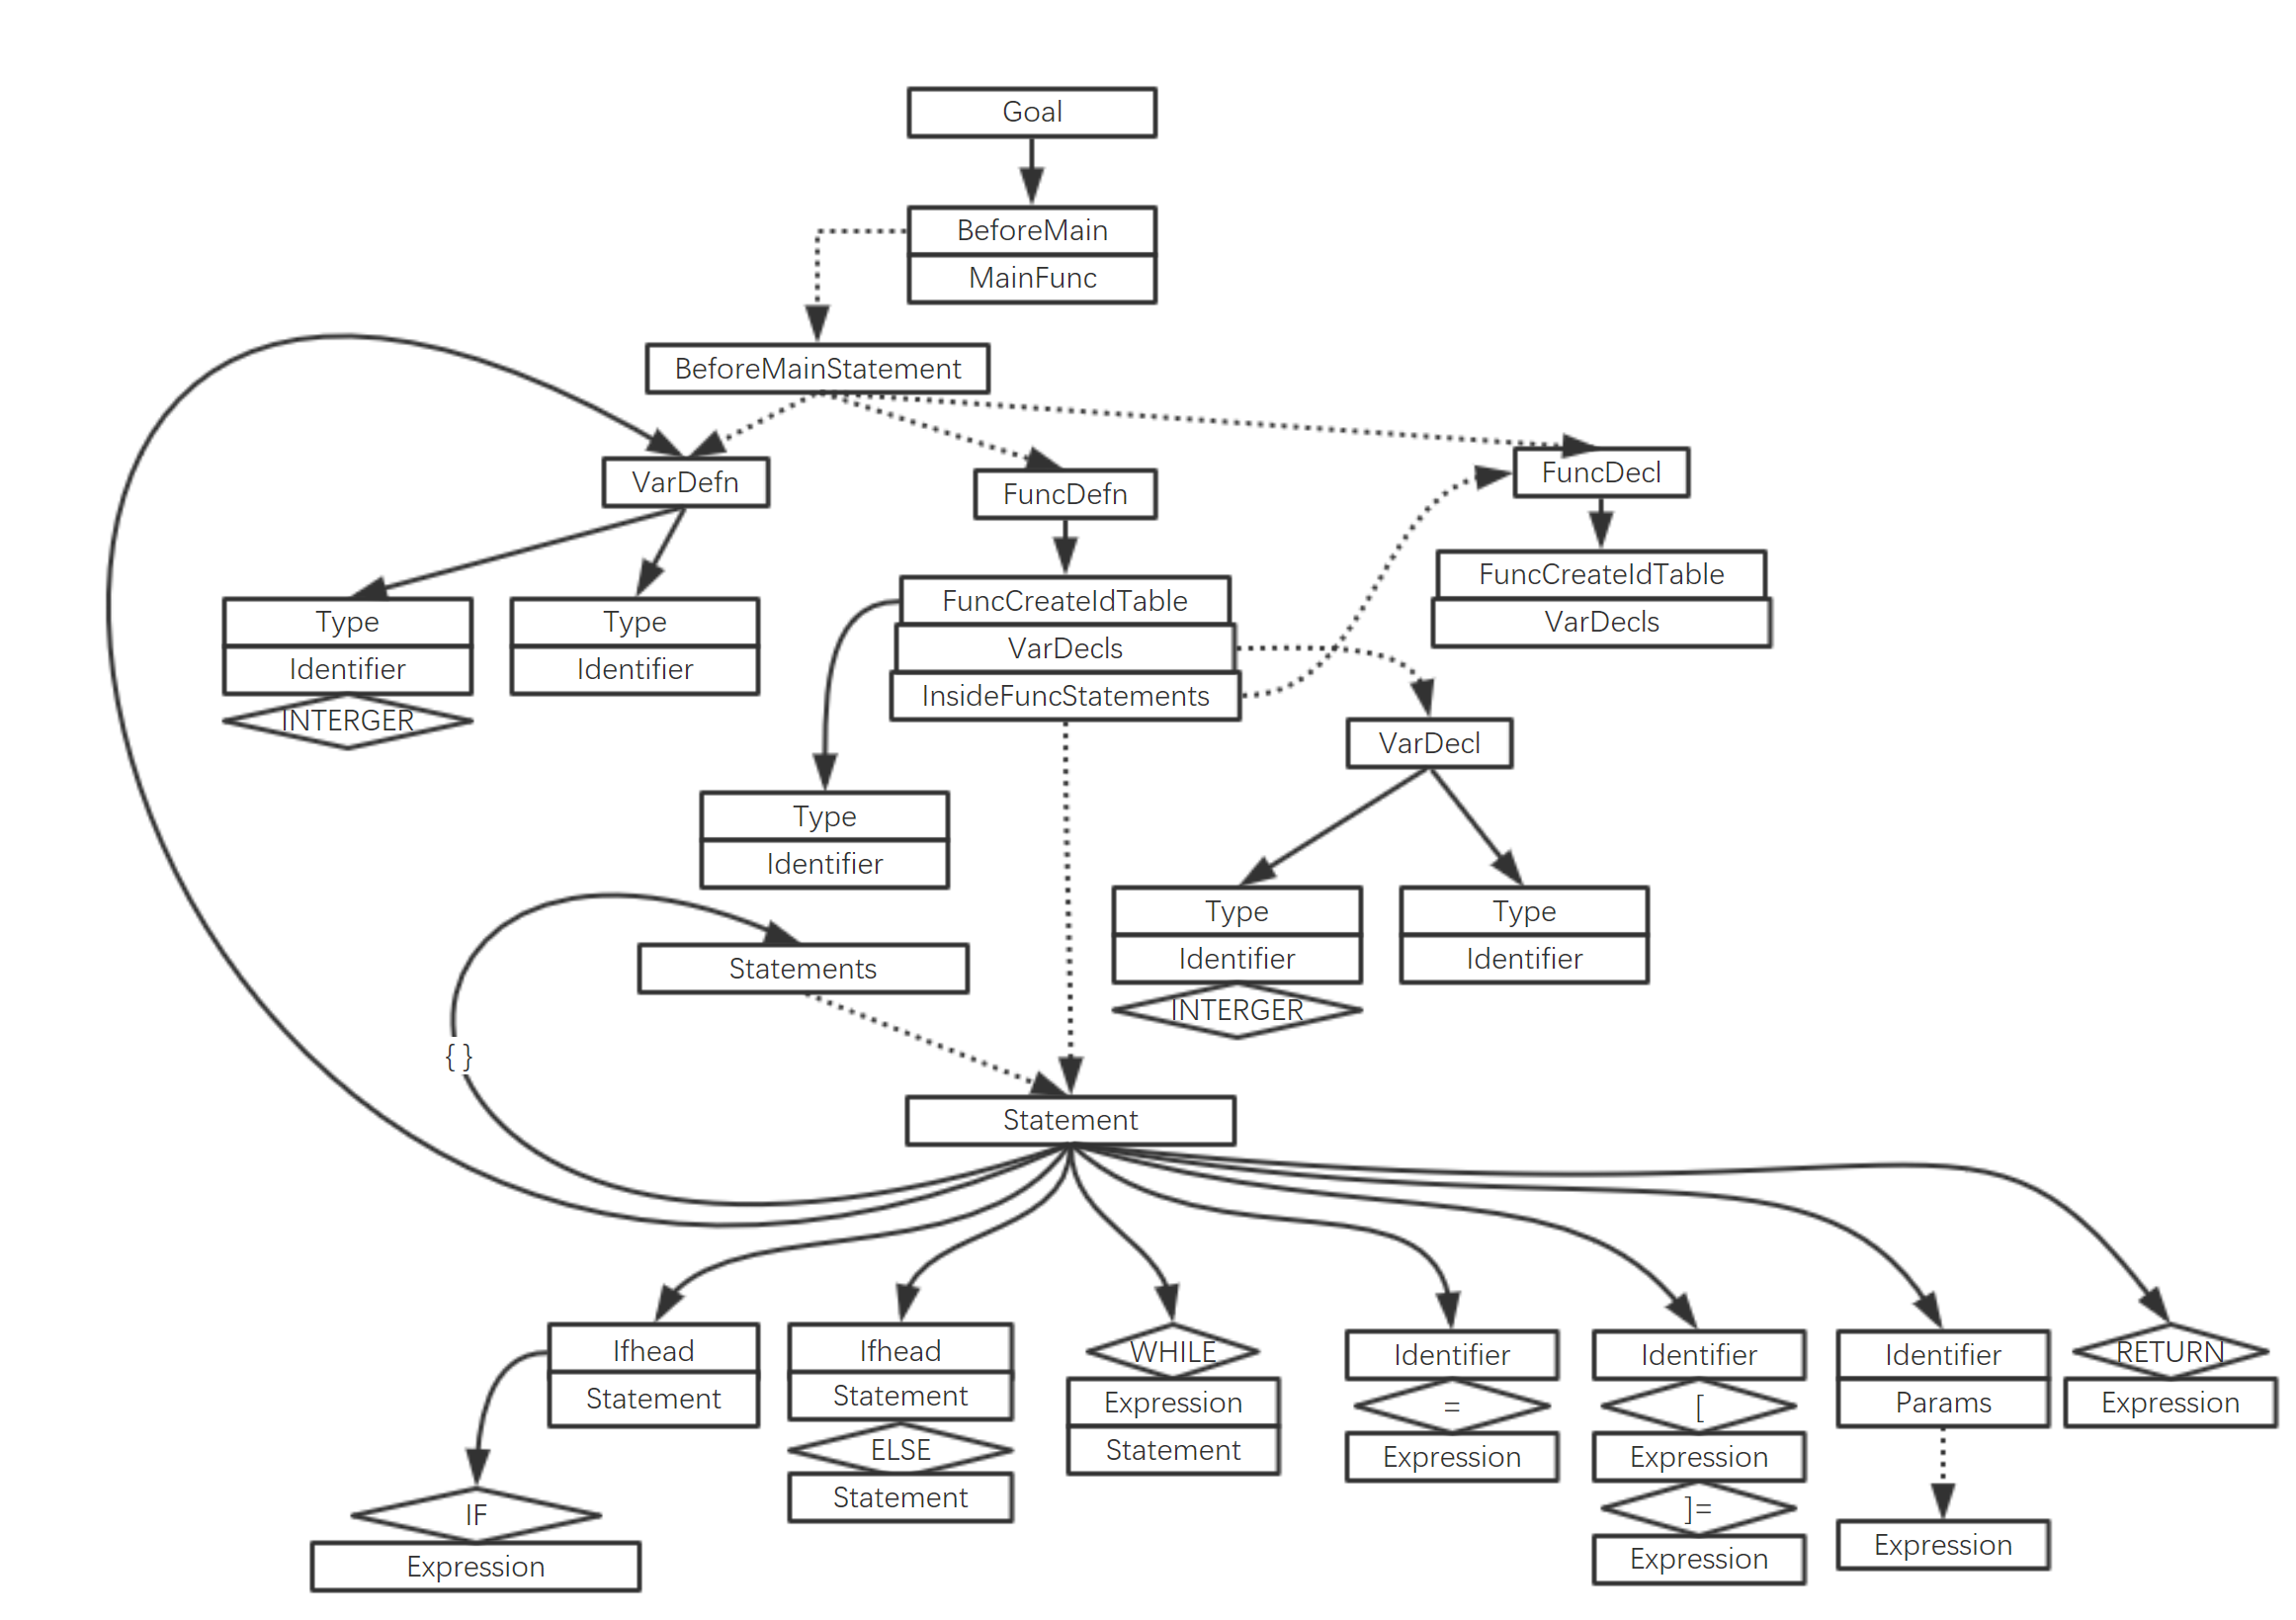
\includegraphics[width=\linewidth]{bnf} 
\end{frame}
\begin{frame}[c]\frametitle{Eeyore 函数声明,定义及参数检查}
\begin{enumerate}[(1)]
\item Declear方法配合decleared属性, 在VarDefn中,调用Declear方法将decleared属性设为true. 在Expression中遇到相应符号时, 需要检查符号的decleared属性,必须是true,否则会报错. 对于函数,Declear方法会存入参数表.
\item Define方法,适用于函数, 作用是声明函数已定义, 若此函数已被声明, 则还需检查此处传入的参数表是否与声明时使用的参数表相匹配,若不匹配则会报错. 但函数声明和定义都不是调用的必要条件, 没有声明的函数也可以直接调用.
\item checkParams方法,检查传入的参数表是否与paramList相匹配. 参数表的类型是Node* ,也就是VarDecl对应的语法树节点. 检查的方法是遍历链表, 检查节点的sym属性的type属性是否对应或可以隐式转换,不匹配的给出错误提示.
\end{enumerate}
\end{frame}
\begin{frame}[c]\frametitle{Eeyore 逻辑表达式和算术表达式转换}
本编译器将比较表达式以及或与非表达式视为逻辑表达式, 五则运算表达式视为算术表达式, 支持逻辑表达式和算术表达式的自动转化.

\begin{enumerate}[(1)]
\item 逻辑表达式转算术表达式: 生成一个临时变量x表示结果,将逻辑表达式的truelist指向运行x=1,然后跳过后面一句x=0;将逻辑表达式的falselist指向运行x=0.
\item 算术表达式转逻辑表达式: 设算数表达式对应的符号为x, 则将该语句翻译为和逻辑比较表达式x==0相同的翻译结果. 即为其生成if-goto-goto语句, 并将truelist初始化为第一个goto对应的序号, 将falselist初始化为第二个goto对应的序号.
\end{enumerate}
\end{frame}
\begin{frame}[c]\frametitle{Tigger 活性分析}
以语句为基本块进行自下而上的活性分析.使用队列进行宽度优先搜索,递推式为:
$$e.in = e.use\cup (e.out - e.def)$$
$$e.out = \cup_{x\in e.nexts} (x.in)$$
如果进行上述计算后e.in和e.out有所改变,则将e的前驱加入队列.

迭代直到队列为空.

\end{frame}
 \begin{frame}[c]\frametitle{Tigger 死代码消除}
此处处理的死代码分为两种:

(1)$e.def \bigcap\left( \bigcup_{x\in e.nexts}x.in \right)== \Phi$ 即该语句定义的变量在这条语句的所有
后继中都不是入口活跃的.

(2)不可达语句,即在活性分析时未处理到的语句.

对于第(1)情行,未定义变量的语句和控制流跳转类语句为例外排除.
\end{frame}
\begin{frame}[c]\frametitle{Tigger 常数传播}
每个Expression语句对象都有一个constant属性,他是一个map表,从变量id映射到该处(出口处)的变量常数值. 此表只会储存此处为常数值的变量.

按顺序遍历所有语句,对于每个语句,计算一个mp(map表)
$$ mp = \bigcap_{x \in e.prevs}x.constant $$
即mp为e的所有前驱的constant表中项的交集,也即对于所有前驱语句都具有相同常数值的变量.

对于非跳转类或访存类语句,如果$ x\in mp \forall x\in e.use $成立,也即所有被x使用的变量在此处均为常数,则可说明此语句定义的变量也为常数. 调用calcarith函数计算此算术运算.并将该语句的类型改为MoveRI(即将直接数赋值给变量的语句)

对于上面公式不成立的语句, 以及跳转类和访存类语句, 令
$$ mp = mp - e.def $$
即此处被定义的变量标记为不是常数.

最后令 $  e.constant = mp $ 记录此语句处的常量表

\end{frame}
\begin{frame}[fragile]\frametitle{Tigger 访存优化}
\begin{lstlisting}
//此处设a保存在栈帧中
c = a + b;
d = a + c;
e = c + d;
\end{lstlisting}
\begin{columns}
\column{.5\textwidth}
优化前的tigger代码:
\begin{lstlisting}
load  0 a0
a1 = a0 + a1
load  0 a0
a1 = a0 + a1
a1 = a1 + a1
\end{lstlisting}
\column{.5\textwidth}
优化后的tigger代码
\begin{lstlisting}
load  0 a0
a1 = a0 + a1
a1 = a0 + a1
a1 = a1 + a1
\end{lstlisting}
\end{columns}

\end{frame}

\begin{frame}[fragile]\frametitle{Tigger 访存优化}
\begin{lstlisting}
b = a + 2;
d = func(1);
d = func(2);
return b;
\end{lstlisting}
\begin{columns}
\column{.5\textwidth}
优化前的tigger代码:
\begin{lstlisting}
a1 = a0 + 2
a0 = 1
store a1 0
call func
load 0 a1
a0 = 2
store a1 0
call func
load 0 a1
a0 = a1
return
\end{lstlisting}
\column{.5\textwidth}
优化后的tigger代码
\begin{lstlisting}
a1 = a0 + 2
a0 = 1
store a1 0
call func
a0 = 2
call func
load 0 a1
a0 = a1
return
\end{lstlisting}
\end{columns}
\end{frame}
\begin{frame}[fragile]\frametitle{Tigger 寄存器分配}
图染色有四种操作:
\begin{enumerate}[1.]
\item 简化:对于度数小于k的传送无关的点,将其从图中删除并放入栈中.
\item 合并:对于一条传送指令,对其关联的两个点在保守规则下合并.
\item 冻结:冻结一条传送指令,将他当作非传送指令.
\item 溢出:将图中度数最大的点放入栈中,并从图中删除.
\end{enumerate}
合并条件:
\begin{enumerate}
\item 对于关联两个普通节点的传送指令,合并这两个节点的条件是:\\如果节点a和b合并产生的节点ab的高度数($\ge K$)的邻节点的个数小于K,则认为a和b的合并是保守的.
\item 对于一个普通节点a和一个预着色节点b的合并,合并条件是:\\对于a的每一个邻接点t,或者t与b已有冲突,或者t是低度数($<K$)节点.
\end{enumerate}
\end{frame}



\end{document}